\subsection{Uncertainty Estimates}
\label{uncertainties}
We discuss here the expected statistical and systematic uncertainties that we expect to contribute to the measurement.

\subsubsection{Systematic Uncertainty}

%An outline of the systematic uncertainty associated with probing small scale spin-1 tensor asymmetry measurements is presented with some plausible
%approaches to minimize the various contributions.  Some details are specific to a solid state polarized target, others are general instrumental issues.  %Using already approved experiments to collect and study systematic effects can be part of an invaluable program to improve the quality of Hall C data taking.

The spin-1 tensor-polarization dependent observables are part of the family of asymmetries which relies on obtaining data for two different target helicity states under equivalent experimental settings.  A large contribution of the experimental uncertainty that effects absolute normalization cancels out as terms in the denominator and numerator are equivalent.  For situations where the experimental configuration has changed during the data collection of the two different helicity states the cancellation does not occur and a rigorous accounting of the errors is required.

The tensor-polarization dependent asymmetry takes the form
\begin{equation}
A_{zz}=\frac{2}{fP_{zz}}\left(\frac{\sigma_p}{\sigma_u}-1\right),
\label{asy}
\end{equation}
where $\sigma_p$ is the polarized cross section and $\sigma_u$ is the unpolarized cross section. There are of course other spin-1 alignment dependent asymmetries, but for positive quadruple polarization in inclusive scattering all polarized observables can be expressed in terms of $A_{zz}$.

The figure of merit (FOM) for a tensor polarized solid state target can be defined as,
\begin{equation}
FOM=n_tf^2P_{zz}^2
\end{equation}
where $n_t$ is the target thickness and $P_{zz}$ is the tensor polarization.




% \paragraph{Systematic Contributions}
The contributions to the experimental uncertainty come from inaccuracies inherent in the system of measurement of the
observable of interest.  Each experiment contains instrumental components of systematic error which may or may not have
dependence on accessible parameters.  These types of errors can have a nonzero mean that changes over time so that its
effect is not reduced when observations are averaged.  There are also stochastic components to the uncertainty which will vary
only around a single mean.  There may still be a time dependence to the standard deviation of the stochastic contributions
but these types of errors can be reliably estimated by repeating measurements.

Monitoring the systemic coupling of the instrumental parameters can greatly reduce the overall uncertainty produced in small asymmetry measurements. An understanding of the evolution of these types of errors over the course of the experiment can be used to make corrections after data acquisition.  Reducing the time in each target spin orientation can also significantly reduce the impact of shifts in normalization.  However, the stochastic components must be regulated prior to and during the experiment.  Helicity flips can not reduce this type of uncertainty contribution.

Many of the errors that arise from limitations in measurement capacity have a statistical probability distribution that can be accurately estimated. 
For many of these types of uncertainties it is possible to derive confidence limits on the domain of the measured value resulting in a relative
contribution to the total systematic error.  Under an independent error assumption these relative contributions add in quadrature, with polarization
being the dominating uncertainty in the spin dependent observables.  The standard law of combination of errors does not work when there are correlations between these types of uncertainties.  For this situation the full covariance matrix is required and a minimization procedure 
maybe needed to keep the error under control.  This is only relevant for dominant errors.  For multiple kinematic tracking variables strict
estimation and handling of each uncertainty is essential for a complete analysis. In many cases one may wish to assume 100\% correlation between variables to simplify the book keeping for smaller contributions.

Errors are often assumed to have a normal distribution.  In reality measurement errors are rarely distributed
in a true Gaussian and usually have some prominent non-Gaussian tail.  Given a sufficient number of measurements the central limit theorem can
be employed to ensure that the estimated parameters will be more Gaussian than the estimated measurements.

Table~\ref{sys-unc} shows a list of the scale dependent uncertainties contributing to the systematic error in $A_{zz}$.

Polarization error is well understood and steps will be taken to minimize these contributions, as has been done in previous experiments~\cite{keller1}.  There are additional uncertainties that can arise from RF quadrupole polarization enhancement, but recent efforts by the UVA target group to study the tensor-enhanced NMR line-shape indicate that the total uncertainty in this case can be held
under 6\% \cite{keller2,keller3}.

\begin{table}
\begin{center}
\begin{tabular}{l|c|c}\hline\hline
Source                         & $A_{zz}$ Systematic & $T_{20}$ Systematic\\
\hline
Polarization                 &   6.0\%  & 6.0\% \\
Dilution factor              &   6.0\%  & 2.5\% \\
Packing fraction             &   3.0\%  & 3.0\% \\
Trigger/Tracking Eff.        &   1.0\%  & 1.0\% \\
Acceptance                   &   0.5\%  & 0.5\% \\
Charge Determination          &  1.0\%  & 1.0\% \\
Detector resolution and efficiency & 1.0\% & 1.0\% \\
\hline
Total  &  9.2\%  & 7.4\% \\
\hline
\end{tabular}
\caption{\label{sys-unc}Estimates of the scale dependent contributions to the systematic error of $A_{zz}$ and $T_{20}$.}
\end{center}
\end{table}

The dilution factor $f$ varies as a function of scattered electron energy, particularly at
kinematics where nucleon resonances are prominent.  The dilution factor must be known precisely at each kinematic point.  This factor must be based on empirical information with measurable error, which will be measured multiple times at each kinematic setting.  Though the loss to the figure of merit can easily be recovered for lower
$f$, the error calculated from the variation of the models is only a crude estimate.

The other uncertainties in Table~\ref{sys-unc} are very standard contributions which are difficult to reduce beyond the listed instrumental lower limit.

\paragraph{Time Dependent Factors}\mbox{}
\label{timedep}

Eq.~\ref{asy} involves the ratio of counts, which leads to cancellation of several first order systematic effects.  However, the fact that the two data sets will not be taken simultaneously leads to a sensitivity to time dependent variations which will need to be carefully monitored and suppressed when possible.  
%
To investigate the systematic differences in the time dependent components of the
integrated counts, the effects from calibration, efficiency, acceptance,
and luminosity between the two polarization states must be considered.
In order to look at the effect on $A_{zz}$ due to drifts in beam current measurement
calibration and detector efficiency, Eq.~\ref{asy} is rewritten explicitly in terms of the raw measured counts $N_1$ and $N$,
\begin{eqnarray} \label{3c}
\nonumber
A_{zz}&=&\frac{2}{fP_{zz}}\left(\frac{N^c_1}{N^c}-1\right) \\
      &=&\frac{2}{fP_{zz}}\left(\frac{Q\varepsilon l \cal{A}}{Q_1\varepsilon_1 l \cal{A}}\frac{N_1}{N}-1\right)
\end{eqnarray}
where $Q$ represents the accumulated charge, and $\varepsilon$ is the detector efficiency. The target length $l$  and acceptance $\cal{A}$ are identical in both states, to first order.

We can then express $Q_1$ as the change in beam current measurement calibration that occurs in
the time it takes to collect data in one polarization state before switching such that $Q_1=Q(1-\delta{Q})$.
In this notation, $\delta{Q}$ is a dimensionless ratio of charges in the different polarization states.  A similar representation
is used for drifts in detector efficiency leading to,
\begin{equation}
A_{zz}=\frac{2}{fP_{zz}}\left(\frac{N_1Q(1-\delta{Q})\varepsilon(1-\delta\varepsilon)}{NQ\varepsilon}-1\right).
\end{equation}
which leads to,
\begin{equation}
A_{zz}=\frac{2}{fP_{zz}}\left(\frac{N_1}{N}(1-\delta{Q}-\delta\varepsilon+\delta{Q}\delta\varepsilon)-1\right).
\end{equation}

Estimates of $\delta{Q}$ and $\delta\varepsilon$ can be obtained from previous experiments.
For the HRS detector drift during the JLab transversity experiment E06-010, the detector response
was measured such that the normalized yield for the same condition over a three month period indicated little change ($<1$\%).
These measurements indicated that for the short time (20 minutes) between target spin flips,
the detector drift should be less than 1\% times the ratio of the time period between target spin flips and three months.
Also considering the period between target polarization states to be
$\approx$12 hours leading to an overall drift $\delta\varepsilon\sim0.01\%$.  A similar approach can be used to establish an estimate
for $\delta{Q}$ using studies from the g2p/GEp experiment, resulting in $\delta{Q}\sim0.01\%$.  The SANE
experiment with a beam current of 100 nA also provides some information. In this case, the relative stability of the current
monitors is on the order of $1\times10^{-3}$, showing oscillations with a period of about an hour.

Expressing $A_{zz}$ in terms of the estimated experimental drifts in efficiency and current measurement,
\begin{equation}
A_{zz}=\frac{2}{fP_{zz}}\left(\frac{N_1}{N}-1\right)\pm\frac{2}{fP_{zz}}\delta\xi.
\end{equation}
where $\delta\xi=\delta{Q}+\delta\varepsilon$. This leads to a contribution to $A_{zz}$ on the order of $1\times10^{-3}$,
\begin{equation}
dA_{zz}^{drift}=\pm\frac{2}{fP_{zz}}\delta\xi=\pm3.7\times10^{-3}.
\end{equation}

Using the standard dilution factor and classically accessible polarization, the precision required in the raw $A_{zz}$ measurement for already-approved DIS $b_1$ experiment is
\begin{equation}
\delta A_{zz}^{raw}=\frac{fP_{zz}}{2}\delta A_{zz} =1.5\times10^{-4}.
\end{equation}
%The polarization state of the target for $b_1$ will be changed a least every 12 hours, so each of the kinematic settings will involve between $N = 12$ to $N = 60$ polarization cycle pairs.

For this proposed $A_{zz}$ measurement, $f$ is changing with $x$ significantly.  For $x\sim1$ the dilution is
greater ($f\sim0.5$) than for the larger $x$ ($f\sim0.1$), where the large signal size indicated by $A_{zz}$ model calculations requires considerably less precision.
The critical point is $x\sim0.8$ where $f$ is less then $0.2$ such that 
\begin{equation}
\delta A_{zz}^{raw}=\frac{fP_{zz}}{2}\delta A_{zz} =\frac{(0.19)(0.2)}{2}(0.05)=1.0\times10^{-3}.
\end{equation}  
So even this most sensitive point is still around an order of magnitude less constrained than the $b_1$ measurement.

Detector efficiencies can drift for a variety of reasons,
including fluctuations in gas quality, high voltage drift, or
drifts in the spectrometer magnetic fields.  All of these types of variation 
can be controlled and minimized during the experiment through careful monitoring as well as systematic studies of the data collected.  
The identical configuration of the two
polarization states minimizes the relative changes in luminosity with respect to time.  
Consistency checks on the measured cross section data can be implemented to 
ensure the quality of each run used in the asymmetry analysis.
Fluctuations in luminosity due to target density variation can be kept to a
minimum by keeping the material beads at the same temperature for both polarization
states through control of the microwave and the liquid helium (LHe) evaporation.  The helium vapor pressure reading
provides an accuracy of material temperature changes at the level of $\sim$0.1\%.
Beam rastering can also be controlled to a high degree.

The dominant source of any variation in acceptance ${\cal A}$ from state to state will be the stability of the target magnetic field.
The capacity to set and hold the target super conducting magnet
to a desired holding field is $\delta B /B=$0.01\%.  The same target cup will be used
for each state, which removes any variation in the target length $l$. 

\paragraph{Drift Mitigation}\mbox{}

Uncertainty in the measuring devices (or resulting normalization deviations) must be small compared to the
scale of the asymmetry at the helicity reversal frequency.  The beam noise that can contribute to these
normalization deviations comes from beam current, beam position, beam energy, beam size (consistent rastering), and beam halo.  Detectors drifts in photomultiplier tube (PMT) gain can change the number of events above
a discriminator threshold, which can become critical when the device PMT behavior changes significantly between
helicity states.  This is also true for drift chamber efficiency, spectrometer analyzing field,
atmospheric pressure and temperature all affect these systems.
The target's superconducting magnet will be operated in persistent current mode, which provides a field uniformity of better than $10^-4$~\cite{Keith:2003ca}. The NMR resonance frequency can also be used to monitor the field with an accuracy exceeding $10^{-5}$.

%The target holding field stability should never be an issue.%, however in $g_2^p$ this proved not to be the case due to a faulty power supply.  Target field instability could certainly destroy data runs taken with under similar defective circumstances.

The most obvious way to improve the experiment considering these contributions is to increase the helicity flip frequency.
Probably the most practiced way to do this is to use two different target cells alternating the cell position between a
polarized target cell and an unpolarized target cell.  By doing this additional uncertainties from using different packing factions,
effective target densities, and target nuclear-chemical compositions are introduced that would not be present when using identical targets for each helicity state.
These contributions maybe able to be mitigated by alternating which cell is polarized.  It is possible to polarize a particular cell
without being in beam having it outside the homogeneous portion of the target field (beam line).  In this way a target cell helicity can be
prepared while taking data on the other cell.  This could potential allow multiple helicity changes in a 24 hour period.

In addition to greater frequency in helicity changes, the initial polarization build-up
can also be enhanced.  It is possible to install an electrically controlled microwave attenuator which will allow a larger amount of microwave power to dump into the target material to speed up polarization.  The attenuator can then be adjusted to the required power to sustain polarization with the addition of the electron beam.  

The uncertainty estimate in charge that results in a small absolute change in the observable is described
in the proposal in the Section~\ref{timedep}.  Analytically there is a component of uncertainty that propagates with the other
relative errors and only a very small piece that results in a drift in the observable.
The resulting expression for the charge and other contributions to the drift in the observable is expressed as,
\begin{equation}
\delta A^d_{zz}=\pm \frac{2}{fP_{zz}}\delta\xi,
\label{drift}
\end{equation}
where $\delta\xi$ contains the sum of $\delta Q$, $\delta \epsilon$, $\delta l$, and $\delta A$.  This means that
to accurately represent $\delta A^d_{zz}$ we must obtain only the residual deviation from the two polarization
states in the time span of a single cycle (sampling of that data point).  The value used for $\delta Q$ is an estimate based
on the actual effect seen in an observable which helps us to separate the relative contribution from the drift in a given time frame.

\paragraph{Trigger-Tracking}
\label{acc}
For the most part, an easy way to determine whether or not drift will lead to an
effect on the error is to determine if the change over time is seen in one polarization state and not the
other with respect to the observable.  Effects from trigger, cuts, and tracking efficiency do lead to errors in normalization,
however both polarization states see the same stochastic fluctuation over the course of a cycle leading only to a small relative uncertainty in the observable.  Aspects of the error that are non-stochastic
and follow an unknown trend have been estimated in the proposal under the name `detector drifts.'
A secondary estimate was obtained based on HRS detector stability using Hall A transversity data for
detected pions.  The resulting drift was $2.2\times10^{-4}$.
The detector thresholds will be set conservatively while using meticulous on-line monitoring and checks to the relative changes in tracking efficiency between slugs.  For our present estimate including trigger, tracking, cuts, and detector errors that show up strictly as contributions to $\delta\xi$, we estimate no larger than $2.2\times10^{-4}$.

\paragraph{Target Dilution and Length}

There are presently UVA designs for target cup and material fabrication to minimize the probability
of changes to target dilution in the form of material loss over time.  The cup contains
multiple hole arrays that are only a 0.1 mm in size.  The material shape and consistency 
is optimized to maximize the packing fraction and minimize the fracturing capacity.  The
ammonia is hand selected to reduce the structural faults to obtain beads approximately 
2 mm in diameter which have already undergone multiple steps of mechanical stress including being pre-irradiated at NIST with a 10 $\mu$A beam.  The temperature
and thus the density of the target is kept the same
in both polarized and unpolarized states.  There are four temperature sensors in a
standard solid polarized target setup that can be used to monitor this.  The temperature
is controlled via LHe evaporation, microwave, and beam heating.  All three are used
to maintain consistent temperature in both polarization states.

The polarized material to be used in the experiment will be contained in 3 cm 
long, 2.54 cm diameter cylinder cups with their axes parallel to the beam.
The cylinders fit inside the 4 cm diameter vertical cylindrical tail piece at 
the bottom of the refrigerator.  The tail piece is full of liquid helium to 
about 20 cm above the beam level.  The heat and radiation of the beam is distributed
uniformly over the cross section of the target normal to the incident beam by a combination
of slow and fast rasters. The fast raster normally is a 2mm by 2mm square shape, traced by the 
sub-millimeter beam at kHz rates.  The slow raster normally is a 1 cm maximum radius spiral, traced at constant tangential speed, covering the rastered area with 5\% dose uniformity at 30 Hz
and can be synchronized to the usual helicity flip signals \cite{chenyan}.

The averaging of the target length done by the rasters results in an effective 
length that is determined by the fraction of the cup volume 
(equivalently, the rastered volume) that is filled with ammonia \cite{chenyan}.
A possible change in the effective target length between the polarized and 
unpolarized periods of a measurement cycle could come from a net change of 
material in the raster volume. Since the raster diameter is 25\% smaller than 
the cup diameter, there is always material outside the raster region that would
fill in an unlikely loss in the rastered region.
A possible estimate of the length change can be obtained by considering the 
ratio of the 0.008 cm$^3$ volume of a fragment to the 6.8 cm$^3$ raster volume 
(including packing fraction) the ratio is $\sim 1/850$.

The only documented instance with ammonia polarized targets and CEBAF $\sim$ 100 
nA beams of a possible rearrangement of material about the target NMR coil that
might indicate an associated net change in material was seen during E07-003 (SANE) which took about 500 hours of $\ge$ 85 nA beam. 
During one 20 h polarized and unpolarized cycle, the loss of 1 or 2 fragments 
would result in a $\sim 1\times 10^{-3}$  change in target length, with a 
$\sim$ 20h/500h probability.
No instances of material fragmentation, which could potentially lead to net 
losses in the raster region have been observed with up to 150 nA CW CEBAF beams 
(E93-026, E01-006, E07-003).  In addition, there are checks in NMR data that can be
used to ensure that no loss of a target fragments occurred between cycles. 

The only instances of material fragmentation for ammonia targets were observed 
at SLAC, in the E143/E155/E155x series of experiments, but the SLAC beam is 
pulsed, with 4 $\mu$s wide pulses of $\sim$20 $\mu$A current at 120 Hz repetition
rate. Such beam time structure can be expected to damage the ammonia crystals by
thermal shock. In fact, to further prevent possible shock effects at JLab, the 
polarized target experiments in Hall C implemented the procedure of gradual
ramping up of the beam current after beam trips.

All changes to the material that occur during movement of the target ladder or
annealing can only happen at the end of each pair of measurement cycles and are
irrelevant for the preceding or following cycles.  Small changes to material
NMR loop coupling are consistent to both polarization states and exist as
a relative error in the polarization.
In addition, as long as the LHe is superfluid ($<2$ K),
its flow can not lead to material rearrangements.  The LHe that is fed
at the bottom of the nose piece coming from the separator is below 2~K, so emptying 
and refilling does not have any effect.

Depolarization using LHe is a relatively standard technique.  In this procedure, the
beam is turned off and the LHe fill valve that controls the
LHe level that surrounds the target insert is slowly reduced as to not replenish
the LHe evaporation until the material has warmed up and the polarization has died out.
The LHe is gradually filled again as in the standard evaporation mode and again set on
automated control.  Once the material is unpolarized and again submerged under
the LHe the microwaves are turned on in off-resonance mode.  The unpolarized target
is then ready for beam.  This procedure provides a quick way to kill polarization while
returning the unpolarized state to the exact condition of the polarized state.  The
small fluctuation in density, temperature and NMR material couple occur in both states
and are a small relative error in the polarization.  All other aspects that may result
in addition to the drift are negligible. 

For example, the target operating temperature is $\sim 1.1\pm 0.15$ K, well below the 
superfluid point.  Over that range, the LHe density, changes by $4\times
10^{-5}$ (the density actually increases below $\simeq 1.1$~K
and increases above, by about equal amounts over the temperature 
interval~\cite{lhe}).
The lattice constant of deuteroammonia~\cite{nd3} changes from 5.048~\AA\ at 2~K to 5.073~\AA\ at 77~K, corresponding to a $1\times 10^{-5}$ change over the 
$\pm$0.15~K interval considered above.  For a 60\% packing fraction, the change 
would be $2.3\times10^{-5}$ for a 0.15~K unexpected temperature difference between
polarization states.
Any possible unaccounted changes in target length between the polarized and 
unpolarized parts of each cycle can also be monitored by recording the time 
dependence of the luminosity with a $\simeq 0.5\times 10^{-4}$ accuracy. %It's our understanding that such device is available in the Hall.

\paragraph{Solid Angle}\mbox{}

The error that arises in the observable due to beam position and magnet currents
over time is inherently very difficult to separate into drift and relative uncertainty.
The 0.1\% error over a 12 hour period is probably quite accurate, however, being
that both polarization states experience the same fluctuations its likely that the majority
of the uncertainty is relative.  There are also concerns on acceptance due to beam position drift. Beam drift
will be monitored during the experiment and accounted for during analysis.  The largest part of this
uncertainty is also a relative contribution to both target states.  The contribution to the drift can be minimized
with the feedback system built for parity experiments
%, which is discussed further in Section~\ref{regress}
.

Trends that arise from dependence of yield on
magnet currents in detectors are a concern related to the spectrometer acceptance.  The drift
effect can be made to be small, for the HRS typically less than $10^{-4}$ for the dipole
and $10^{-3}$ for the three quads, and similarly for the HMS.  The effects on the acceptance can be determined and
corrected through careful analysis.  Naturally, the
target magnet current does not need to be changed between cycles, as the uniformity, stability, and setability
pointed out in the proposal eliminate field variation between the two polarization
states.  The residual drift from solid angle effects after such correction is expected to be no larger than 0.01\%.
This value was already accounted for in Section \ref{acc}.

\iffalse
\paragraph{Multivariate Regression}\mbox{}
\label{regress}

The error that arises in the observable due to drifts in beam current or position, analyzing magnet currents,
and many others can depend on many parameters that may be available such as instrument temperature, gas levels in spectrometer,
ambient conditions in the Hall, etc.  This type of information can be made part of the data stream and can be used in a regression
analysis to understand the change in the normalization components between the different helicity states.  A correction can then
be made mitigating the false asymmetry from that specific deviation.
\begin{figure}
\begin{center}
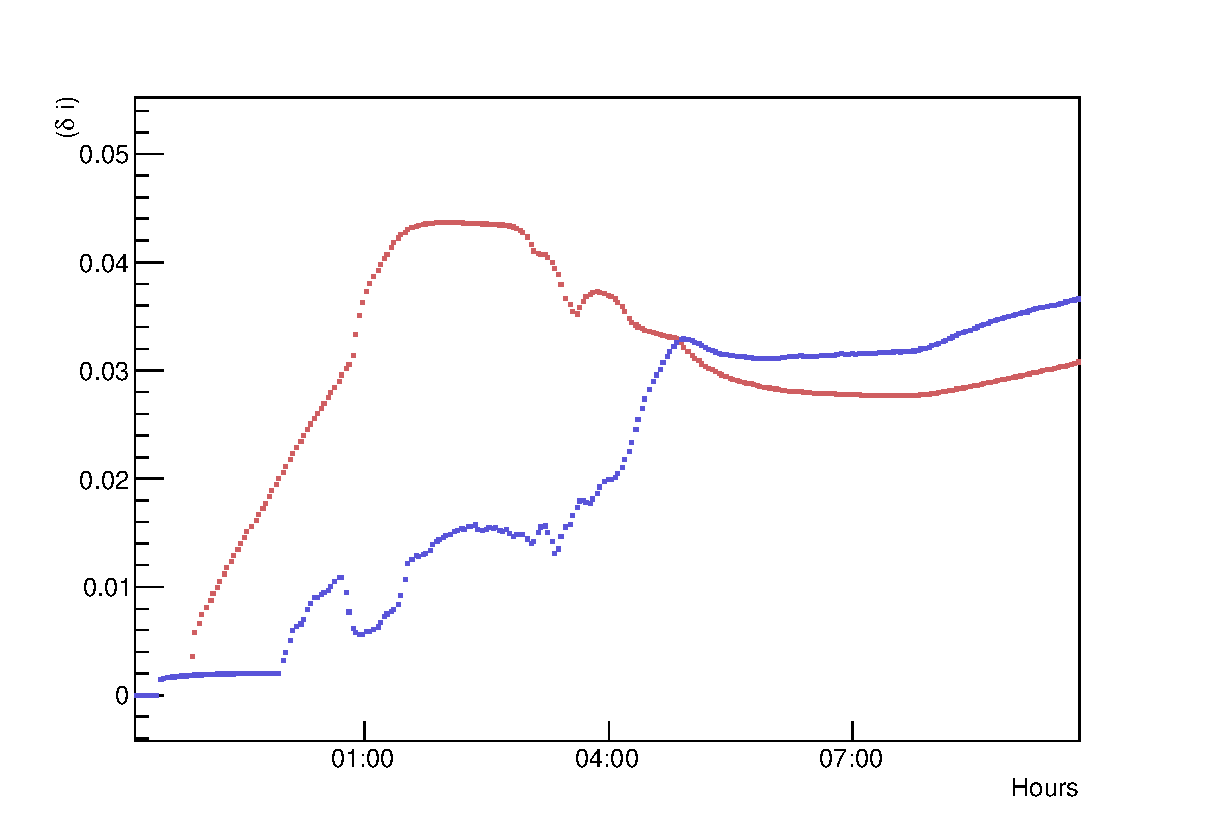
\includegraphics[height=75mm, angle=0]{./figs/dev}
\end{center}
\caption{Hypothetical deviation of the two Hall C beam current monitors.}
\label{dev}
\end{figure}
Figure \ref{dev} show a hypothetical deviation of the two Hall C BCM.  The $y$-axis is the current percent deviation in a BCM affected by temperature changes
evolving in time.  This is for a demonstration only and is a simulation based on
data taken from previous experiments.  The simulation incorporates a systemic coupling
to temperature which could be reconstructed using a multivariate regression.

Figure \ref{qweak} shows the ratio of the two standard Hall C beam current monitors over a 40 hour period during the Q-weak experiment.  The
variation in the two beam current monitors is thought to have a strong dependence on monitor unit temperature.  Having a measurement of temperature of each
monitor over time gives additional information that can be used to model the dynamic behavior of the beam current deviations.  

\begin{figure}
\begin{center}
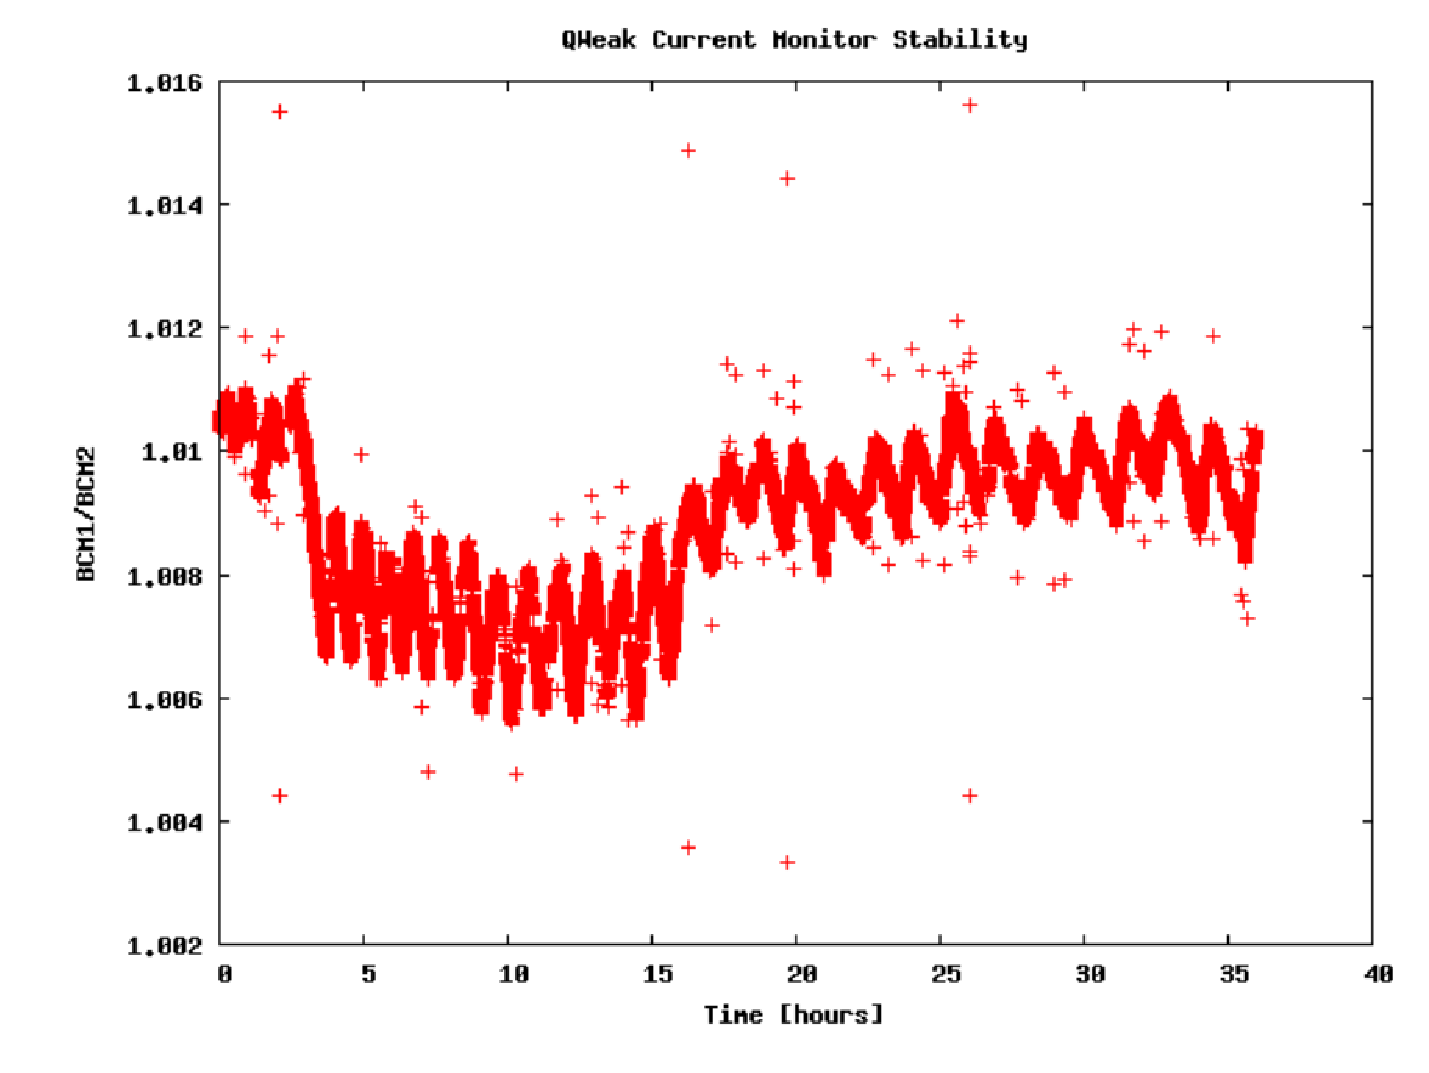
\includegraphics[height=75mm, angle=0]{./figs/qweak}
\end{center}
\caption{The ratio of the two standard Hall C beam current monitors over a 40 hour period during the Qweak experiment.}
\label{qweak}
\end{figure}

To use an example with real data, consider the polarization normalization changes as a function of the Q-meter.  There are linear scaling effects that
lead to a shift in the DC-offset as well as nonlinear contributions that effect the systems capacity to measure accurately.  These effects are a function
of both time and temperature.  A simple regression using a linear model is used based on the deviation seen in polarization at different temperature, as shown in Fig. \ref{PolTemp}.
The model can be used to correct the polarization given any temperature of the Q-meter NMR.  The nonlinear effects are not seen as a function of temperature as much as a
function of time.  This is likely because certain parts of the circuit heat up at different rates having separate but correlated effects.  The basic linear model can be
improved by simply adding the time-stamp into the data-stream and running a multivariate analysis using polarization, time and temperature.  Figure \ref{regression} show
four different trials using a Artificial Neural Network and well as a Boosted Decision Tree.  The $y$-axis shows $g(T)$ average deviation (with error bar showing the spread of deviation) from the true value and the measured/correct value.  From the left each point reflects no correction, linear model correction, multivariate regression using temperature, and multivariate regression using temperature and time, respectively, as part of the feature space. 
\begin{figure}
\begin{center}
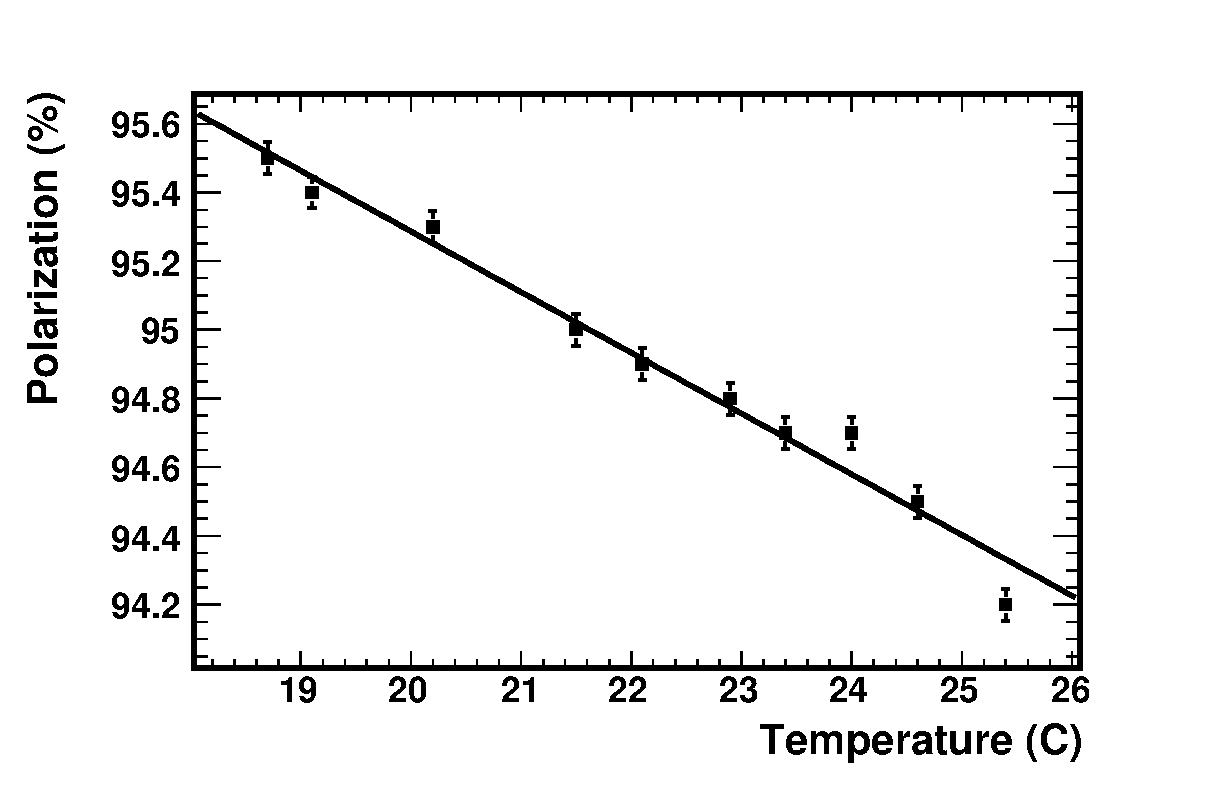
\includegraphics[height=75mm, angle=0]{./figs/PolTemp}
\end{center}
\caption{A simple regression using a linear model is used based on the deviation seen in polarization at different temperature}
\label{PolTemp}
\end{figure}

It is possible to measure the change in an element of drift with respect to other parameters.  Measurements of this systemic coupling
can be used to disentangle effects that are driven by changes in the environment over time.  For example, knowledge of luminosity monitors or BCM temperature
can be used in regression to account for changes in the values.  Drifts that change as a function of some quantifiable parameter can be understood
and corrected if that parameter is also recorded in time.  This type of empirical information taken over several experiments can be invaluable 
for the experiments to follow.  This is exceedingly true with the use of multivariate regression where multiple variables over multiple experiments can be used to train a learning algorithm to interpret various environmental contributions and deduce the effects on essential covariance trends.  %More research would be needed to implement these techniques in the modern experimental hall infrastructure.

\begin{figure}
\begin{center}
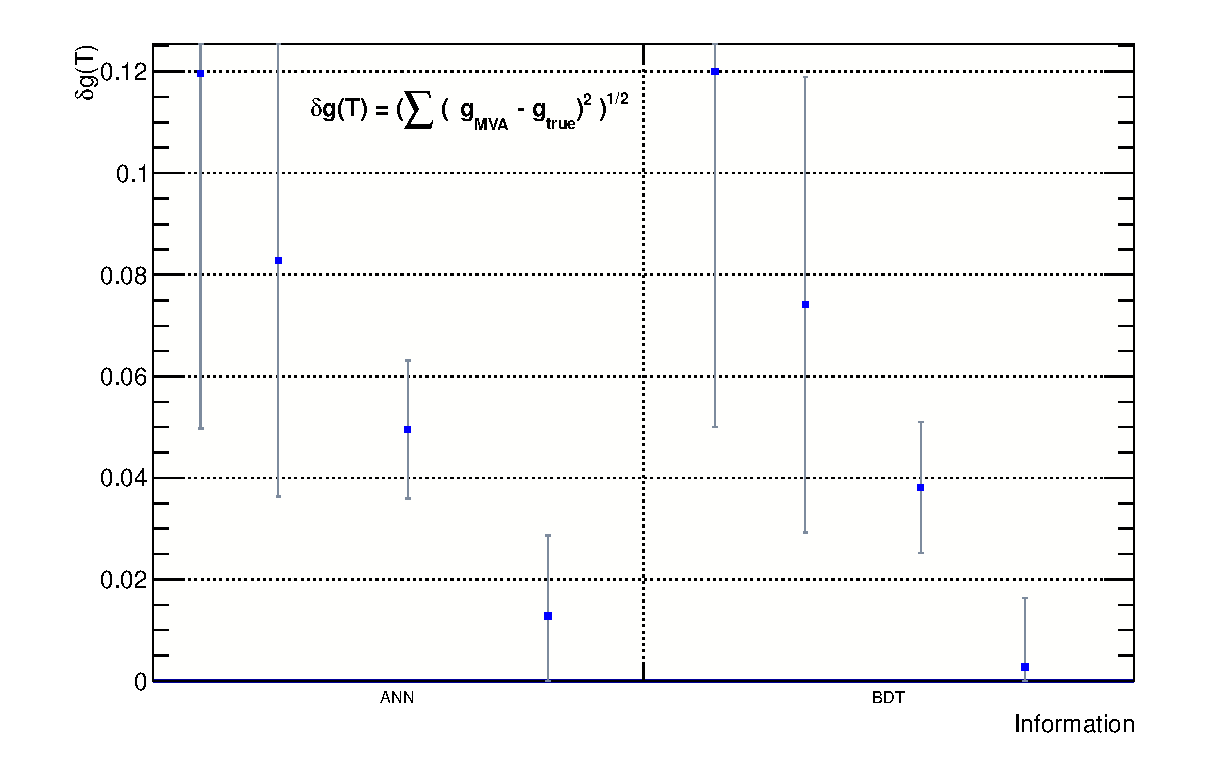
\includegraphics[height=75mm, angle=0]{./figs/Regression}
\end{center}
\caption{Average deviation for the (from left) no correction, linear model correction, multivariate regression using temperature, and multivariate regression using temperature and time as part of the feature space.  The left (right) plot uses an Artificial Neural Network (Boosted Decision Tree) as the multivariate algorithm.}
\label{regression}
\end{figure}
\fi


\paragraph{Beam Current Monitors}\mbox{}

Information has been extracted from experiment E06-010 for high current (10-15 $\mu$A),
in which all the systematics are included in the yield studies including detector
drift, acceptance drift, BCM drift and acceptance due to BPM drift.
The beam charge asymmetries between two helicity states using the luminosity monitors for experiment E06-010 has been shown to be at the level of $4\times10^{-5}$ with a width of $2.3\times10^{-4}$.  An additional estimate on the change in the BCM calibration
constant is seen in experiment E08-027 resulting in a absolute deviation of $2.0\times10^{-4}$ over the course
of six days.  Long term drifts can be reduced by careful thermal isolation of the BCMs, however resulting trends will be need to be studied and corrections implemented.  
%It should be considered a priority to monitor and correct for remaining temperature dependence.

Fluctuations in the calibration of beam current measuring devices can be well understood
and mitigated.  Even when calibrations are taken frequently, a small change in the BCM response over
the course of a single helicity flip iteration can contribute a drift on the order of $1\times10^{-4}$.
%As mentioned previously,
A Boosted Decision Tree regression maybe used similar to that used for the temperature dependence
of the Q-meter.  This would require accurate temperature monitoring of the BCM stainless steel pillbox
resonant cavity in operation.  Creating a heat regulating system using a fluid circulated chiller could
help to both stabilize and accurately measure the temperature.  Additional temperature stabilization of analog cables, and optimizing cable length maybe also help.


\iffalse
\paragraph{Multivariate Dilution Factor}
The change in dilution as a function of $x$ must be known very well.  The uncertainty based
on the variation in models is likely to be grossly underestimated.  If not, and the models
accurately reflect the change in dilution around the $x \approx 1$ and resonance regions, it maybe
possible to extract a near background free set of counts reducing the effective dilution
that goes into the asymmetry calculation.  Using a reliable model or direct empirical information
it is possible to train a Boosted Decision Tree (BDT) to discriminate between the different various
contributions to the spectrum.  Though it is for a two arm experiment, this type of procedure was
suggested for the UVA real Compton scattering experiment (RCS) \cite{Day}.  Using only one arm implies a
great reliance on the model of the dilution, which will likely always be a weak point in this
experiment even with the application of advance techniques.  It is unclear how well this could
work for $A_{zz}$ but I can mention some highlights from RCS.

For the real Compton initial state helicity correlations asymmetry, a photon and proton are detected.
It is not trivial to obtain data free of background events. However, it is possible to obtain
data free of signal events, by selecting different regions of the $\delta X$ and $\delta Y$ phase
space, so that accurate numbers can be obtained for the asymmetry of
pion events. It is then possible to measure the asymmetry for pure background events, the asymmetry for mixed
RCS-background events, and the fraction of the latter events that are RCS.  The latter number is
has a direct effect on the dilution factor in the polarized asymmetry calculation.
Each step can contribute to the error in the resulting RCS asymmetry on both a systematic 
and statistical level.  To consider a technique of
directly extracting the real Compton events negating the need for the asymmetry for mixed
RCS-background events a Monte Carlo simulation is used.  The RCS single events and $\pi^0$ background
events are generated and used to train the multivariate algorithm. 

The result of analysis from the training
of the boosted decision tree indicating the response of the classifier is shown in the left plot.
The real Compton signal resolving efficiency as a function of the cut on the BDT response can be understood using
multiple iterations of the Monte Carlo along with Signal efficiency and background efficiency.  The optimal cut is determined by
using the derivative of the significance function $S/\sqrt{S+B}$.
The classifier response indicated that even with the only three mentioned
discriminating variable it is possible to obtain greater then 98\% signal
when making a constraint on the BDT response to eliminate the pion
background.  The separation using a Monte Carlo demonstration is shown in Fig.~\ref{fig:d11}  
\begin{figure}[h]
\begin{center}
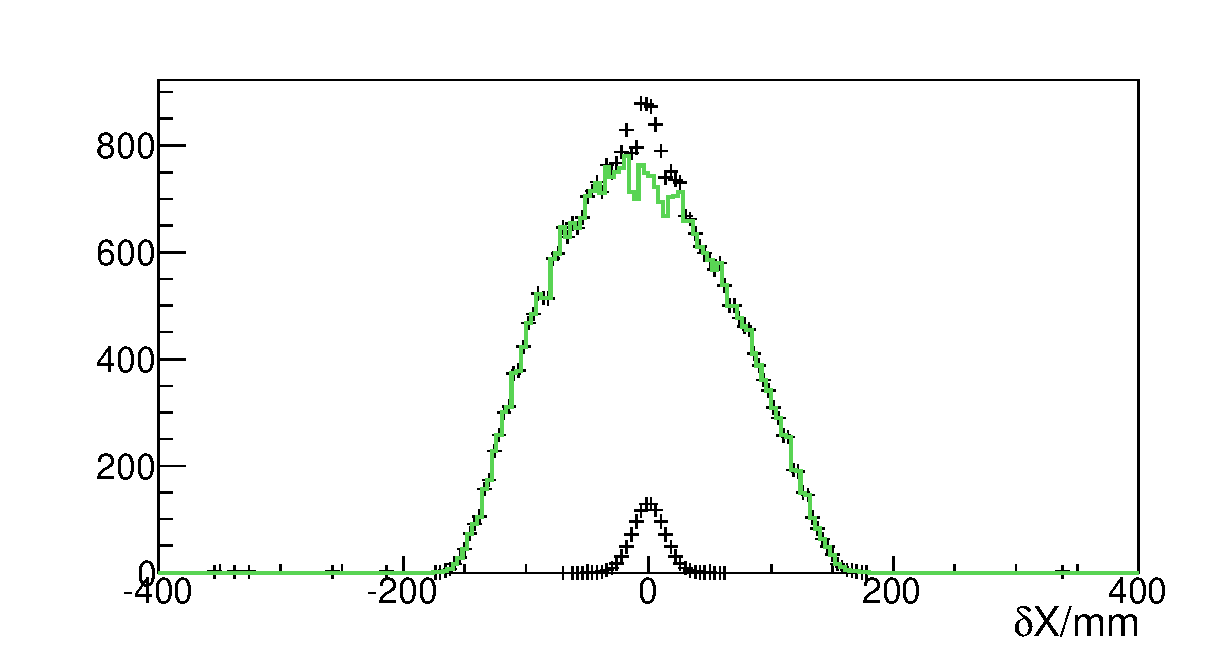
\includegraphics[height=75mm, angle=0]{./figs/d11}
\caption{The $\delta X$ distribution with signal and background before separation and after.
The result of imposing the optimal BDT response cut at 0.063 leading to a RCS event extraction
with 98\% signal efficiency.  This demonstrates a separation with 1000 Compton events and 10000 $\pi^0$ background events.
This is only a Monte Carlo demonstration.}
\label{fig:d11}
\end{center}
\end{figure}

This technique is especially useful for situations in which the background
is difficult to distinguish from the signal in the spectra.  Through the use of multivariate
discrimination of the phase space even a small signal that is nearly
unrecognizable among the background can be separated out with a well defined
uncertainty associated with it.
\fi

\paragraph{Systematic Summary}\mbox{}


It is essential to consider each uncertainty and each source separately as well as understand systemic coupling.  
This proposed $A_{zz}$ measurement would be a great benefit to understand and minimize systematic uncertainties for small asymmetry measurements such as $b_1$. Having data at a large range of beam
current, energy, and target types while studying beam noise and detector stability can help to build a comprehensive map of critical systematic issues. Other systematic minimization techniques can be explored during $A_{zz}$ in addition to the systematic minimization mentioned in this proposal, which will be critical for $b_1$~\cite{Keller:2015tn} and could help many other future experiments. In fact there is no better experimental opportunity to study the systematics of probing asymmetries in Hall C then $A_{zz}$ at high $x$. Because of the scale of the predicted asymmetry $A_{zz}$ for large $x$, the drifts that can corrupt
$b_1$ are only relevant for the lower $x$ points, although for $A_{zz}$ in this region a systematic error of the order of ($1\times10^{-3}$) would be very good, which has an order of magnitude more leeway
then for $b_1$. 



\iffalse
\subsubsection{Systematic Uncertainty}% in $A_{zz}$ }
\begin{table}
\begin{center}
\begin{tabular}{l|c}\hline\hline
Source								& Systematic \\
\hline
$P_{zz}$ Polarimetry					& 12\%   \\
Dilution Factor						& 6.0\%   \\
Packing Fraction						& 3.0\%   \\
Trigger/Tracking Efficiency			& 1.0\% \\
Acceptance							& 0.5\% \\
Charge Determination					& 1.0\%  \\
Detector Resolution and Efficiency	& 1.0\% \\
\hline
Total								& 14\%   \\
\hline
\end{tabular}
\caption{\label{error1}Estimates of the scale dependent contributions to the systematic error of $A_{zz}$.}
\end{center}
\end{table}

Table \ref{error1} shows a list of the scale dependent uncertainties contributing to the systematic error in $A_{zz}$.
With careful uncertainty minimization in polarization the relative error in vector polarization, $Pz$, can be less than or equal to 3.9\%, as was demonstrated for the proton in the recent E08-027/E08-007 experiment~\cite{NIMDUST} and nearly as good for the deuteron using multiple techniques to measure the NMR signal as discussed in ~\cite{PTSTDUST}.  With the use of a positive tensor enhanced target it has been projected to be able to achieve a relative error in $P_{zz}$ better than 12\% ~\cite{PTSTDUST}.  The uncertainty from the dilution in the polarized target is estimated to be
about 6\% over the range of kinematics points of interest.  We consider separately the uncertainty in the packing fraction of the ammonia target contributes at a level of less than 3\%. Charge calibration and detector efficiencies are expected to be known better to 1\%. 
%but the impact of time-dependent drifts in these quantities must be carefully controlled.

\subsubsection*{Time Dependent Systematic Effects}
Eq.~\ref{3} involves the ratio of counts, which leads to cancellation of several first order systematic effects.  However, the fact that the two data sets will not be taken simultaneously leads to a sensitivity to time dependent variations which will be monitored and suppressed. The typical size of these types of effects are small compared to the large asymmetries predicted for most of the proposed kinematic regions, but must be carefully monitored whenever the expected asymmetry is small, such as at a zero crossing.

%While typical false asymmetries in Hall C of $0.1\%$ are acceptable for this proposed measurement, we are interested in a strict control of the systematics for further reduction.
%
To investigate the systematic differences in the time dependent components of the integrated counts, we need to consider the effects from calibration, efficiency, acceptance, and luminosity between the two polarization states.

Fluctuations in luminosity due to target density variation can easily be kept to a minimum by keeping the material beads at the same temperature for both polarization states by control of the microwave and the LHe evaporation.  The He vapor pressure reading gives accuracy of material temperature changes at the level of $\pm0.1\%$.
%Beam rastering can also be controlled to a high degree.

The beam charge asymmetries between two helicity states using the luminosity monitors for experiment
E06-010 has been shown to be at the level of $4 \times 10^{-5}$ with a width of $2 \times 10^{-4}$.
An additional estimate on the change in the BCM calibration constant is seen in
experiment E08-027 resulting in a absolute deviation of $2 \times 10^{-4}$ over the course of six
days. We expect to be able to minimize long term drifts by careful thermal isolation of
the BCMs.
%, however resulting trends will be studied and corrections implemented.

The acceptance of each cup can only change as a function of time if the magnetic field changes.  
The capacity to set, reset, and hold the target superconducting magnet to a desired holding field causes a field uncertainty of $\delta B /B=0.01\%$. 
This implies that, like the cup length $l$, the acceptance ${\cal A}$ for each polarization state is the same.

In order to look at the effect on $A_{zz}$ due to drifts in beam current monitor calibration and detector efficiency, we rewrite Eq.~\ref{3} explicitly in terms of the raw measured counts $N_p^c$ and $N_u^c$,
\begin{eqnarray} \label{3c}
\nonumber
A_{zz}&=&\frac{2}{fP_{zz}}\left(\frac{N^c_p}{N^c_u}-1\right) \\
      &=&\frac{2}{fP_{zz}}\left(\frac{Q\varepsilon l \cal{A}}{Q_1\varepsilon_1 l \cal{A}}\frac{N_p}{N_u}-1\right)
\end{eqnarray}
where $Q$ represents the accumulated charge, and $\varepsilon$ is the detector efficiency. The target length $l$ and acceptance $\cal{A}$ are identical in both states to first order.

We can then express $Q_1$ as the change in beam current measurement calibration that occurs in
the time it takes to collect data in one polarization state before switching to another, such that $Q_1=Q(1-dQ)$.
In this notation, $dQ$ is a dimensionless ratio of changes in different polarization states and would ideally be equal to zero.  A similar representation
is used for drifts in detector efficiency leading to,
\begin{equation}
A_{zz}=\frac{2}{fP_{zz}}\left(\frac{N_pQ(1-dQ)\varepsilon(1-d\varepsilon)}{N_u Q\varepsilon}-1\right).
\end{equation}
which simplifies to,
\begin{equation}
A_{zz}=\frac{2}{fP_{zz}}\left(\frac{N_p}{N_u}(1-dQ-d\varepsilon+dQd\varepsilon)-1\right).
\end{equation}

We obtain estimates of $dQ$ and $d\varepsilon$ from previous experimental
studies.  During the JLab transversity experiment E06-010, the detector drift was measured such that the normalized yield over a three month period indicated little change ($<1$\%).
These measurement were then used to show that for short time (20 minutes periods between target spin flip),
the detector drift was estimated to be less than 1\% times the ratio of the time period between target spin flip and three months.
For the present experiment we use the same estimate except for the period between target polarization states used is
$\approx 36$ hours leading to an overall drift $d\varepsilon\approx 0.01\%$.  A similar approach is used to establish an estimate
for $dQ$ using studies from the data from the E08-027 experiment resulting in $d\varepsilon \approx 0.01\%$.

To express $A_{zz}$ in terms of the estimated experimental drifts in efficiency and current measurement we can write,
\begin{equation}
A_{zz}=\frac{2}{fP_{zz}}\left(\frac{N_1}{N}-1\right)\pm\frac{2}{fP_{zz}}d\xi.
\end{equation}
This leads to a contribution to $A_{zz}$ on the order of $1\times10^{-3}$,
\begin{equation}
dA_{zz}^{drift}=\pm\frac{2}{fP_{zz}}d\xi=\pm3.7\times10^{-3}.
\end{equation}
%For this estimate we assume only two polarization state changes in a day. If it is possible to increase this rate then the systematic effect in $A_{zz}$ will decrease accordingly.

Naturally detector efficiency can drift for a variety of reasons, for
example including fluctuations in gas quality, HV drift or
drifts in the spectrometers magnetic field.  All of these types of variation as can be realized both
during the experiment though monitoring as well as systematic studies of the data collected.
Checks on the consistency of the cross section data that can be use ensuring the quality of each run will be used in the asymmetry analysis.  Regression can be use to correct for any long term drifts that are of a non-stochastic nature.
Each of these systematic effects can mitigate the systematic uncertainty to $\sim0.001$. 
In the kinematic region proposed here, $A_{zz}$ is expected to be large, on the order of $0.1$ to $1.0$, making any absolute errors on this scale only critical as the data and models pass through the x-axis.  

\fi

\subsubsection{Statistical Uncertainty}
\label{stat}
To investigate the statistical uncertainty we start with the equation for $A_{zz}$ using
measured counts for polarized data ($N_p$) and unpolarized data ($N_u$), 
\begin{equation}
A_{zz}=\frac{2}{fP_{zz}}\left(\frac{N_p}{N_u}-1\right).
\end{equation}
The statistical error with respect to counts is then
\begin{equation}
\delta A_{zz}=\frac{2}{fP_{zz}}\sqrt{\left(\frac{\delta N_p}{N_u}\right)^2+\left(\frac{N_p\delta N_u}{N_u^2}\right)^2}.
\end{equation}
For $\delta N_{p(u)}=\sqrt{N_{p(u)}}$, the uncertainty becomes
\begin{equation}
\label{dAzz}
\delta A_{zz}=\frac{2}{fP_{zz}}\sqrt{\frac{N_p(N_u + N_p)}{N_u^3}},
\end{equation}
which can't be simplified further due to the large expected asymmetry.

The number of counts was calculated using a combination of P. Bosted's~\cite{Bosted:2012qc} and M. Sargsian's~\cite{misak-convo} code for $x<2$. The Bosted code was used for the lowest $Q^2$ setting, where effects of SRC scaling are expected to be negligible, and for $x<1.1$ to accurately determine the quasi-elastic peak. The Sargsian code was used for the higher $Q^2$ settings at $x>1.1$ due to its inclusion of SRC scaling effects.

The deuteron elastic peak was calculated using a parametrization of the deuteron elastic form factors $A$ and $B$ by

\begin{equation}
\frac{d^2 \sigma}{d\Omega dE'} = \sigma_{\mathrm{Mott}}\left(\frac{E'}{E}\right)\left[ A + B \tan ^2 \left( \frac{\theta}{2} \right) \right] \delta (E'-E'_{el}),
\end{equation}

where $\delta(E'-E'_{el})$ is approximated by a Gaussian distribution with its width determined by the resolution of the spectrometers, 
\begin{equation}
\delta(E'-E'_{el}) = \frac{1}{2\Delta E\cdot E'_{el}\sqrt{\pi}}e^{-\frac{(E'-E'_{el})^2}{2(\Delta E\cdot E'_{el})^2}}, 
\end{equation}
where $\Delta E=0.1 ~(0.08)\%$ for the HMS (SHMS) and $E'_{el}=\frac{Q^2}{2m_D}.$ This was added to the rates calculation that was used for quasi-elastic $A_{zz}$ and $b_1$~\cite{Long:2013tn}, and the uncertainty of $A_{zz}$ on the elastic peak was calculated the as in Eq.~\ref{dAzz}.

Following the methodology discussed in Section~\ref{t20_exp}, to obtain statistical uncertainties for $T_{20}$ we scale our calculated elastic $A_{zz}$ uncertainties by
\begin{equation}
\delta t_{20} = \sqrt{2}\delta A_{zz}.
\end{equation}

The projected uncertainties for $A_{zz}$ are summarized in Tables~\ref{RATES2}-\ref{RATES3} and displayed in Figs.~\ref{PROJ}-\ref{PROJ-zoom}. The projected uncertainties for $T_{20}$ are summarized in Table~\ref{RATES-T20} and displayed in Fig.~\ref{PROJ-T20}.  






\begin{table}
\begin{center}
\begin{tabular}{c|ccc|ccc|ccc}
 ~ & \multicolumn{3}{|c}{H1: $Q^2=2.9\mathrm{~(GeV/}c)^2$} & \multicolumn{3}{|c}{H2: $Q^2=1.8\mathrm{~(GeV/}c)^2$} & \multicolumn{3}{|c}{S1: $Q^2=1.5\mathrm{~(GeV/}c)^2$} \\
 \hline
  $x$  & $f_{dil}$ & $\delta A_{zz}^{stat}$ & $\delta A_{zz}^{sys}$ & $f_{dil}$ & $\delta A_{zz}^{stat}$ & $\delta A_{zz}^{sys}$ & $f_{dil}$ & $\delta A_{zz}^{stat}$ & $\delta A_{zz}^{sys}$ \\
  &     & $\times 10^{-2}$  & $\times 10^{-2}$  &    & $\times 10^{-2}$  & $\times 10^{-2}$ &    & $\times 10^{-2}$  & $\times 10^{-2}$ \\
\hline\hline
%       |         Q2=2.9         |      Q2=1.8           |      Q2=1.5
%  x  	   fdil 	   dAzz	 dAzzSys  fdil 	  dAzz   dAzzSys  fdil   dAzz	 dAzzSys
 0.50   &  0.29	 & 2.02	& 1.84	& ---	& ---	& ---	& 0.25	& 0.72	& 1.84 \\
 0.60   &  0.29	 & 0.91	& ????	& 0.27	& 3.15	& ????	& 0.30	& 0.36	& ???? \\ 
 0.70   &  0.27	 & 1.01	& ????	& 0.32	& 1.26	& ????	& 0.29	& 0.38	& ???? \\
 0.80	&  0.30	 & 1.11	& 1.34	& 0.20	& 2.00	& 0.48	& 0.17	& 0.74	& 1.34 \\
 0.90	&  0.24	 & 1.73 	& 0.38 	& 0.27	& 1.45	& 1.10	& 0.29	& 0.44	& 0.38 \\
 1.00	&  0.46	 & 1.03	& ???? 	& 0.50	& 0.74	& ????	& 0.51	& 0.24	& ???? \\
 1.10	&  0.28	 & 2.48	& 0.14 	& 0.33	& 1.58	& 1.65	& 0.34	& 0.49	& 0.14 \\
 1.20	&  0.09	 & 11.7	& 1.55 	& 0.10	& 7.18	& 3.31	& 0.17	& 1.34	& 1.55 \\
 1.30	&  0.11	 & 16.8	& 4.13 	& 0.11	& 9.76	& 4.96	& 0.12	& 2.79	& 4.13 \\
 1.40	&  ---	 & ---	& --- 	& 0.12	& 15.1	& 6.65	& 0.13	& 4.30	& 6.72 \\
 1.50	&  ---	 & ---	& ---	& 0.11	& 19.8	& 8.29	& 0.10	& 7.01	& 8.34 \\
 1.60	&  ---	 & ---	& --- 	& ---	& ---	& ---	& 0.10	& 9.60	& 8.42 \\
 1.70	&  ---	 & ---	& --- 	& ---	& ---	& ---	& 0.10	& 12.7	& 7.04 \\
 1.80	&  ---	 & ---	& --- 	& ---	& ---	& ---	& 0.10	& 16.6	& 4.72 \\
 2.00   &  ---	 & ---	& ---	& 0.20	& 9.33	& 9.20	& 0.50	& 2.79	& 9.20 \\
\hline\hline
\end{tabular}
\caption{\label{RATES2}Summary of the expected uncertainty for each $x$ bin for settings S1, H1, and H2. }
\end{center}
\end{table}

\begin{table}
\begin{center}
\begin{tabular}{c|ccc|ccc|ccc}
 ~ & \multicolumn{3}{|c}{S2: $Q^2=0.7\mathrm{~(GeV/}c)^2$} & \multicolumn{3}{|c}{H3: $Q^2=0.3\mathrm{~(GeV/}c)^2$} & \multicolumn{3}{|c}{S3: $Q^2=0.2\mathrm{~(GeV/}c)^2$} \\
 \hline
  $x$  & $f_{dil}$ & $\delta A_{zz}^{stat}$ & $\delta A_{zz}^{sys}$ & $f_{dil}$ & $\delta A_{zz}^{stat}$ & $\delta A_{zz}^{sys}$ & $f_{dil}$ & $\delta A_{zz}^{stat}$ & $\delta A_{zz}^{sys}$ \\
  &     & $\times 10^{-2}$  & $\times 10^{-2}$  &    & $\times 10^{-2}$  & $\times 10^{-2}$ &    & $\times 10^{-2}$  & $\times 10^{-2}$ \\
\hline\hline
%       |         Q2=0.7         |      Q2=0.3           |      Q2=0.2
%  x  	   fdil 	   dAzz	 dAzzSys  fdil 	  dAzz   dAzzSys  fdil   dAzz	 dAzzSys
 0.30   &  0.24	 & 0.99	& 1.84	& ---	& ---	& ---	& 0.18	& 2.13	& 1.84 \\
 0.40   &  0.28	 & 0.26	& 1.84	& ---	& ---	& ---	& 0.12	& 1.38	& 1.84 \\
 0.50   &  0.32	 & 0.21	& 1.84	& 0.14	& 3.52	& 1.84	& 0.11	& 1.23	& 1.84 \\
 0.60   &  0.19	 & 0.41	& ????	& 0.12	& 2.26	& ????	& 0.18	& 0.78	& ???? \\ 
 0.70   &  0.13	 & 0.68	& ????	& 0.18	& 1.33	& ????	& 0.28	& 0.48	& ???? \\
 0.80	&  0.19	 & 0.48	& 0.48	& 0.30	& 0.72	& 0.48	& 0.42	& 0.31	& 0.48 \\
 0.90	&  0.39	 & 0.22 	& 1.10 	& 0.46	& 0.45	& 1.10	& 0.54	& 0.24	& 1.10 \\
 1.00	&  0.52	 & 0.16	& ???? 	& 0.52	& 0.43	& ????	& 0.58	& 0.25	& ???? \\
 1.10	&  0.39	 & 0.28	& 1.27 	& 0.43	& 0.63	& 1.07	& 0.53	& 0.33	& 0.95 \\
 1.20	&  0.22	 & 0.65	& 2.54 	& 0.30	& 1.15	& 2.14	& 0.40	& 0.55	& 1.91 \\
 1.30	&  0.14	 & 1.34	& 3.81 	& 0.19	& 2.16	& 3.22	& 0.32	& 0.83	& 2.87 \\
 1.40	&  0.09	 & 2.29	& 5.06 	& 0.14	& 3.52	& 4.29	& 0.24	& 1.31	& 3.82 \\
 1.50	&  0.06	 & 4.09	& 6.35	& 0.10	& 5.85	& 5.37	& 0.20	& 1.86	& 4.78 \\
 1.60	&  0.04	 & 7.76	& 7.60 	& 0.06	& 10.4	& 6.45	& 0.14	& 2.87	& 5.74 \\
 1.70	&  0.04	 & 9.23	& 8.88 	& 0.05	& 13.5	& 7.52	& 0.10	& 4.53	& 6.69 \\
 1.80	&  0.03	 & 14.9	& 9.20 	& 0.06	& 13.9	& 8.60	& 0.11	& 4.73	& 7.66 \\
 2.00   &  0.67	 & 3.79	& 9.20	& 0.20	& 3.05	& 9.20	& 0.70	& 0.45	& 9.20 \\
\hline\hline
\end{tabular}
\caption{\label{RATES3}Summary of the expected uncertainty for each $x$ bin for settings S2, S3, and H3. }
\end{center}
\end{table}


\begin{figure}
\begin{center}
%\includegraphics[width=0.45\textwidth]{figs/plots0705/b1_proj_newmiller_lin.eps}
%\hspace{0.5cm}
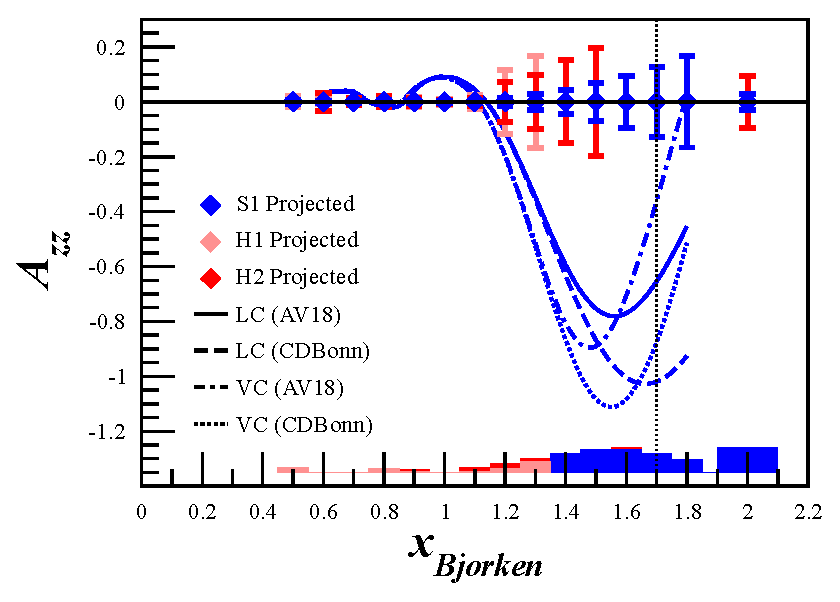
\includegraphics[width=0.49\textwidth]{figs/Azz_S1_H1_H2_vn_lc.eps} 
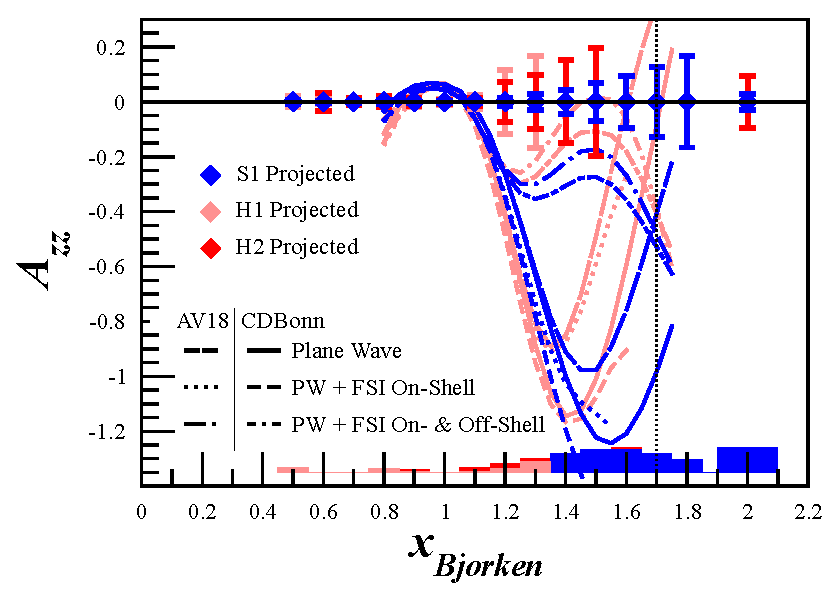
\includegraphics[width=0.49\textwidth]{figs/Azz_S1_H1_H2_fsi.eps} \\
\includegraphics[width=0.49\textwidth]{figs/Azz_S2_H3_S3.eps} 
\caption{\label{PROJ}Projected uncertainties for the tensor asymmetry $A_{zz}$ with \productiondays days of beam time. The band represents the systematic uncertainty. The top row shows the $Q^2>1.0~(\mathrm{GeV}/c)^2$ settings and the bottom row shows the $Q^2<1.0~(\mathrm{GeV}/c)^2$. The upper $x$ limit for H1 (H2) is $x=1.3$ ($x=1.5$). The upper-left plot includes light-cone (LC) and virtual-nucleon (VN) calculations provided by M. Sargsian~\cite{Sargsian:2014fla}, as well as the dependence of each model on various deuteron wave functions (AV18, CDBonn). The dotted line at $x=1.75$ indicates the threshold of $W_{NN}>m_D+100$~MeV where LC and VN calculations begin to not be valid as $A_{zz}$ approaches the elastic peak. The upper-right plot includes virtual-nucleon plane wave and final state interaction (FSI) calculations provided by W. Cosyn~\cite{cosyn-convo}. The bottom row includes a modified Frankfurt and Strikman model~\cite{Frankfurt:1988nt} that estimates the peak shifts in $x$ expected due to the SRC scaling changing with $Q^2$~\cite{Frankfurt:2008zv}.
}
\end{center}
\end{figure}

\begin{figure}
\begin{center}
%\includegraphics[width=0.45\textwidth]{figs/plots0705/b1_proj_newmiller_lin.eps}
%\hspace{0.5cm}
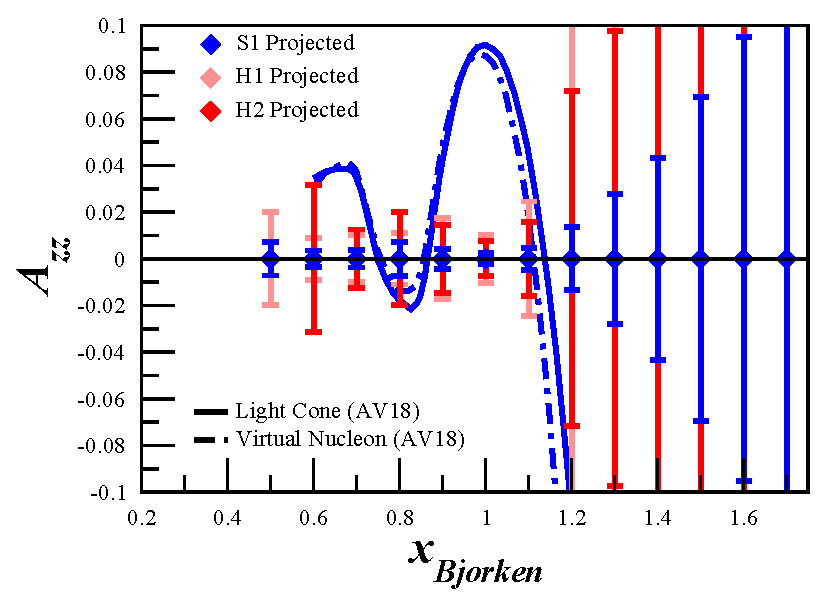
\includegraphics[width=0.49\textwidth]{figs/Azz_S1_H1_H2_zoom.eps} 
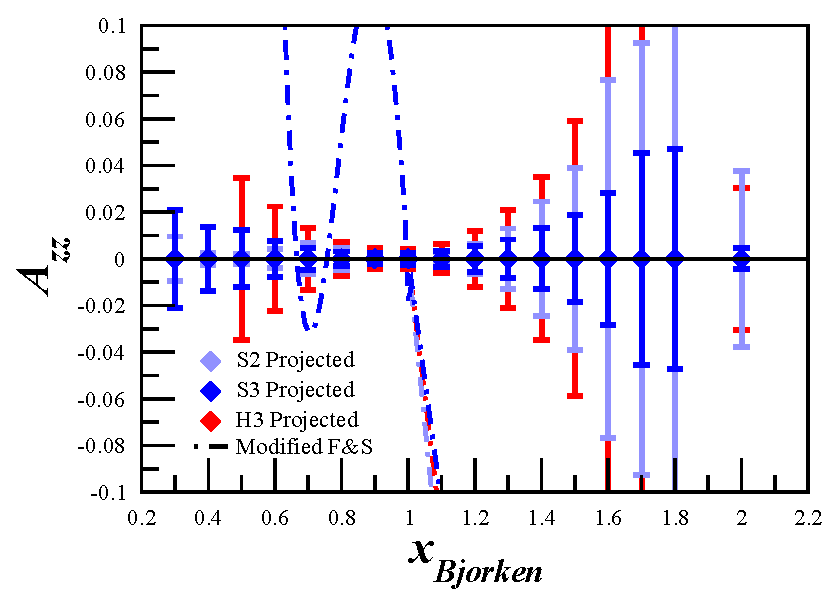
\includegraphics[width=0.49\textwidth]{figs/Azz_S2_H3_S3_zoom.eps} 
\caption{\label{PROJ-zoom}Projected uncertainties for the tensor asymmetry $A_{zz}$ with \productiondays days of beam time, same as in Figure~\ref{PROJ}, but zoomed in to $-0.1<A_{zz}<0.1$ to more clearly show the small uncertainties around the quasi-elastic peak.
}
\end{center}
\end{figure}

\begin{table}
\begin{center}
\begin{tabular}{c|c|c|c}
		& $Q^2$    	& $\delta T_{20}^{stat}$	&  $\delta T_{20}^{sys}$ \\
Setting	& (GeV$^2$)	& $\times 10^{-2}$		& $\times 10^{-2}$ \\
\hline\hline
H2 		& 1.8		&  13.2					& 4.7 \\  
S1 		& 1.5		&  3.95					& 4.6 \\
S2 		& 0.7		&  5.36					& 4.6 \\  
H3 		& 0.3		&  4.31					& 9.2 \\  
S3 		& 0.2		&  0.64					& 5.5 \\
  
\hline\hline
\end{tabular}
\caption{\label{RATES-T20}Expected uncertainties for $T_{20}$, assuming a systematic uncertainty of 9.2\%, which could be reduced further by utilizing the S3 measurement as a calibration for the polarized target.}
\end{center}
\end{table}

\begin{figure}
\begin{center}
%\includegraphics[width=0.45\textwidth]{figs/plots0705/b1_proj_newmiller_lin.eps}
%\hspace{0.5cm}
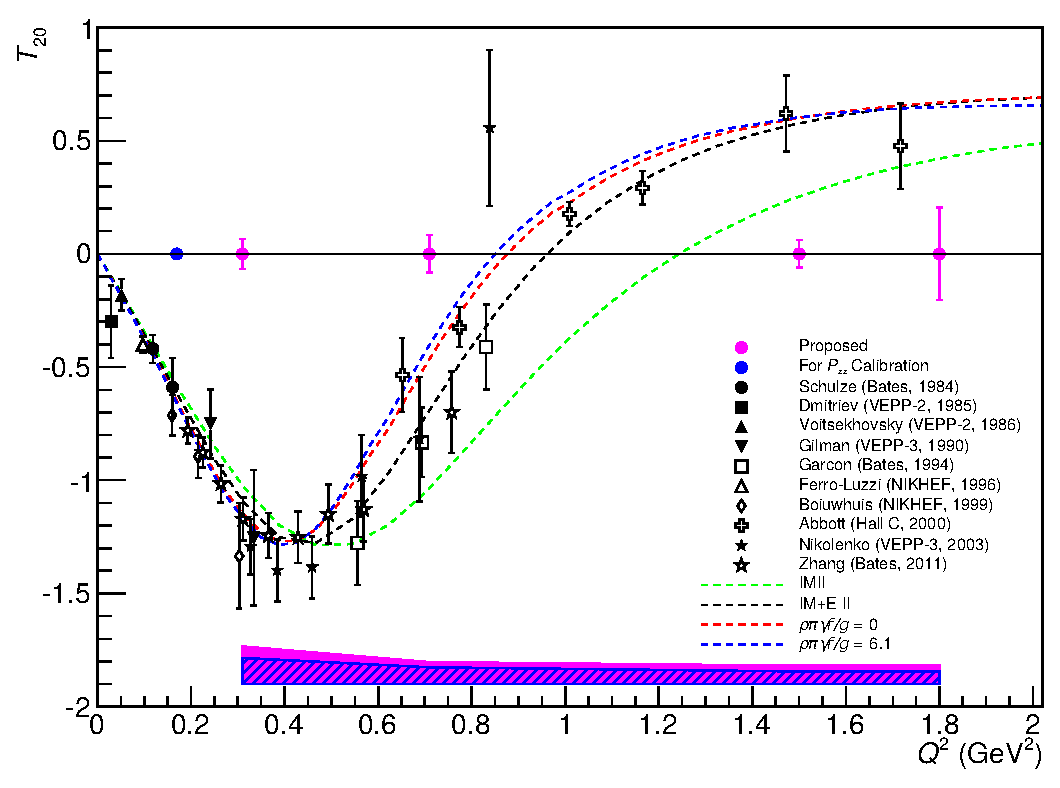
\includegraphics[width=\textwidth]{figs/plot_t20_fit.eps} 
\caption{\label{PROJ-T20}Projected statistical uncertainties for the elastic tensor analyzing power $T_{20}$ with \productiondays days of beam time.
}
\end{center}
\end{figure}